\scanpage{77}
% letterhead
\begin{center}
{\sffamily INSTITUT\\
DES HAUTES ÉTUDES SCIENTIFIQUES}\\[-0.4ex]
\rule{1.7cm}{0.5pt}
\end{center}

\figure{\footnotesize\begin{tikzpicture}
\node[anchor=west,inner sep=0pt,align=left] (haut) at (0,0) {
\(\overline{\underline{\unsure{\mathrm{VI}|\mathrm{VII}}}}\,
 1.11\ \text{\unsure{:|à}}\ 1.14\
 \text{\unsure{apres|après}}\ 1.15\,-\,\unsure{1.22|1.21}\ \text{? Refaire }1.14\ \text{?}\)\\[1.3ex]
\(\overline{\underline{\mathrm{VI}}}\)\quad appendice : la lettre Deligne 2 pages};
\draw[semithick] ([xshift=-.15em,yshift=.18ex]haut.north west)
 .. controls +(-.29em,-.26ex) and +(.12em,.50ex) .. ([xshift=-.28em,yshift=.79ex]haut.west)
 .. controls +(.12em,-.62ex) and +(.26em,.22ex) .. ([xshift=-.64em]haut.west)
 .. controls +(.49em,-.17ex) and +(.05em,.44ex) .. ([xshift=-.26em,yshift=-.82ex]haut.west)
 .. controls +(.02em,-.46ex) and +(-.23em,-.13ex) .. ([xshift=-.1em,yshift=-.1ex]haut.south west);
% A second lower contour is visible in the retraced brace.
\draw[thin] ([xshift=-.08em,yshift=.16ex]haut.west)
 .. controls +(-.18em,-.30ex) and +(-.15em,.50ex) .. ([xshift=-.04em,yshift=-.13ex]haut.south west)
 .. controls +(.05em,-.16ex) and +(.12em,-.05ex) .. ([xshift=.03em,yshift=-.02ex]haut.south west);
\node[inner sep=0pt] (sga) at ([xshift=-1.15cm,yshift=-.4ex]haut.west) {SGA 7};
\draw[thin] ([xshift=-.79cm,yshift=-.06cm]sga.center)
 .. controls +(.07cm,.45cm) and +(-.47cm,.03cm) .. ([xshift=.72cm,yshift=.64cm]sga.center)
 .. controls +(.04cm,-.47cm) and +(.38cm,.03cm) .. ([xshift=-.18cm,yshift=-.65cm]sga.center)
 .. controls +(-.40cm,0cm) and +(-.05cm,-.24cm) .. ([xshift=-.79cm,yshift=-.06cm]sga.center);
\end{tikzpicture}}

% slanted
\reversemarginpar\margin{\raisebox{-1.4\baselineskip}[0pt][0pt]{\shortstack[l]{faire un\\exposé\\\(\overline{\underline{\mathrm{XXIII}}}\) ?}}}\normalmarginpar
\figure{\footnotesize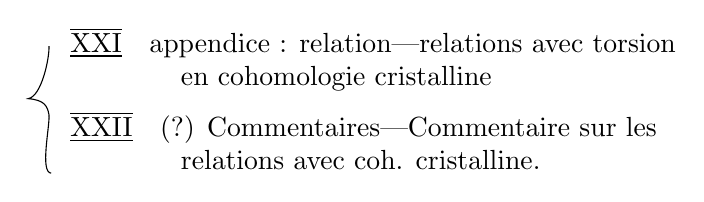
\begin{tikzpicture}
\node[anchor=west,inner sep=0pt,align=left] (bas) at (0,0) {
 \(\overline{\underline{\mathrm{XXI}}}\)\quad appendice : \unsure{relation|relations} avec torsion\\
 \hspace{4em}en cohomologie cristalline\\[1.5ex]
 \(\overline{\underline{\mathrm{XXII}}}\)\quad (?) \unsure{Commentaires|Commentaire} sur les\\
 \hspace{4em}relations avec coh. cristalline.};
\draw[thin] ([xshift=-.75em,yshift=-1.6ex]bas.north west)
 .. controls +(.02em,-1.0ex) and +(.48em,.18ex) .. ([xshift=-1.5em]bas.west)
 .. controls +(.6em,-.12ex) and +(-.06em,.72ex) .. ([xshift=-.75em,yshift=-1.35ex]bas.west)
 .. controls +(.04em,-.9ex) and +(-.42em,.05ex) .. ([xshift=-.67em,yshift=-.25ex]bas.south west);
\end{tikzpicture}}
% archive sheet number: 76
